%% For double-blind review submission, w/o CCS and ACM Reference (max submission space)
\documentclass[sigplan,review,anonymous]{acmart}\settopmatter{printfolios=true,printccs=false,printacmref=false}
%% For double-blind review submission, w/ CCS and ACM Reference
%\documentclass[sigplan,review,anonymous]{acmart}\settopmatter{printfolios=true}
%% For single-blind review submission, w/o CCS and ACM Reference (max submission space)
%\documentclass[sigplan,review]{acmart}\settopmatter{printfolios=true,printccs=false,printacmref=false}
%% For single-blind review submission, w/ CCS and ACM Reference
%\documentclass[sigplan,review]{acmart}\settopmatter{printfolios=true}
%% For final camera-ready submission, w/ required CCS and ACM Reference
%\documentclass[sigplan]{acmart}\settopmatter{}


%% Conference information
%% Supplied to authors by publisher for camera-ready submission;
%% use defaults for review submission.
\acmConference[PL'18]{ACM SIGPLAN Conference on Programming Languages}{January 01--03, 2018}{New York, NY, USA}
\acmYear{2018}
\acmISBN{} % \acmISBN{978-x-xxxx-xxxx-x/YY/MM}
\acmDOI{} % \acmDOI{10.1145/nnnnnnn.nnnnnnn}
\startPage{1}

%% Copyright information
%% Supplied to authors (based on authors' rights management selection;
%% see authors.acm.org) by publisher for camera-ready submission;
%% use 'none' for review submission.
\setcopyright{none}
%\setcopyright{acmcopyright}
%\setcopyright{acmlicensed}
%\setcopyright{rightsretained}
%\copyrightyear{2018}           %% If different from \acmYear

%% Bibliography style
\bibliographystyle{ACM-Reference-Format}
%% Citation style
%\citestyle{acmauthoryear}  %% For author/year citations
%\citestyle{acmnumeric}     %% For numeric citations
%\setcitestyle{nosort}      %% With 'acmnumeric', to disable automatic
                            %% sorting of references within a single citation;
                            %% e.g., \cite{Smith99,Carpenter05,Baker12}
                            %% rendered as [14,5,2] rather than [2,5,14].
%\setcitesyle{nocompress}   %% With 'acmnumeric', to disable automatic
                            %% compression of sequential references within a
                            %% single citation;
                            %% e.g., \cite{Baker12,Baker14,Baker16}
                            %% rendered as [2,3,4] rather than [2-4].


%%%%%%%%%%%%%%%%%%%%%%%%%%%%%%%%%%%%%%%%%%%%%%%%%%%%%%%%%%%%%%%%%%%%%%
%% Note: Authors migrating a paper from traditional SIGPLAN
%% proceedings format to PACMPL format must update the
%% '\documentclass' and topmatter commands above; see
%% 'acmart-pacmpl-template.tex'.
%%%%%%%%%%%%%%%%%%%%%%%%%%%%%%%%%%%%%%%%%%%%%%%%%%%%%%%%%%%%%%%%%%%%%%


%% Some recommended packages.
\usepackage{times}
\usepackage{t1enc}
\usepackage{todonotes}
\usepackage{graphicx}
\usepackage{epstopdf}
\usepackage{hyperref} % hyperlinks for references.
\usepackage{amssymb,amsmath,amsthm,amsfonts} % easier math formulae, align, subequations \ldots
\usepackage[vlined,ruled]{algorithm2e}
\usepackage{array}
\usepackage{rotating}
\usepackage{booktabs}
\usepackage{color}
\usepackage{caption}
\usepackage{subcaption}
%\usepackage{algorithm}
\usepackage{algorithmic}
\usepackage{wrapfig}



\usepackage{verbatim}
\usepackage{multirow}

\usepackage{lscape}

\usepackage{fancyhdr}

\usepackage{booktabs}   %% For formal tables:
                        %% http://ctan.org/pkg/booktabs
\usepackage{subcaption} %% For complex figures with subfigures/subcaptions
                        %% http://ctan.org/pkg/subcaption
                        
   \begin{document}                     

\newcommand{\pluseq}{\mathrel{+}=}
\newcommand{\asteq}{\mathrel{*}=}

\makeatletter
\newcommand{\heading}[1]% #1 = text
{\par\vskip 1.5ex \@plus .2ex
 \hangindent=1em
 \noindent\makebox[1em][l]{$\,\bullet$}\textbf{\large #1}%
\par\vskip 1.5ex \@plus .2ex
\@afterheading}
\makeatother

\newif\ifcmts
\cmtstrue % comment out to hide answers


%\begin{document}

%% Title information
\title[Short Title]{Full Title}         %% [Short Title] is optional;
                                        %% when present, will be used in
                                        %% header instead of Full Title.
\titlenote{with title note}             %% \titlenote is optional;
                                        %% can be repeated if necessary;
                                        %% contents suppressed with 'anonymous'
\subtitle{Subtitle}                     %% \subtitle is optional
\subtitlenote{with subtitle note}       %% \subtitlenote is optional;
                                        %% can be repeated if necessary;
                                        %% contents suppressed with 'anonymous'


%% Author information
%% Contents and number of authors suppressed with 'anonymous'.
%% Each author should be introduced by \author, followed by
%% \authornote (optional), \orcid (optional), \affiliation, and
%% \email.
%% An author may have multiple affiliations and/or emails; repeat the
%% appropriate command.
%% Many elements are not rendered, but should be provided for metadata
%% extraction tools.

%% Author with single affiliation.
\author{First1 Last1}
\authornote{with author1 note}          %% \authornote is optional;
                                        %% can be repeated if necessary
\orcid{nnnn-nnnn-nnnn-nnnn}             %% \orcid is optional
\affiliation{
  \position{Position1}
  \department{Department1}              %% \department is recommended
  \institution{Institution1}            %% \institution is required
  \streetaddress{Street1 Address1}
  \city{City1}
  \state{State1}
  \postcode{Post-Code1}
  \country{Country1}                    %% \country is recommended
}
\email{first1.last1@inst1.edu}          %% \email is recommended

%% Author with two affiliations and emails.
\author{First2 Last2}
\authornote{with author2 note}          %% \authornote is optional;
                                        %% can be repeated if necessary
\orcid{nnnn-nnnn-nnnn-nnnn}             %% \orcid is optional
\affiliation{
  \position{Position2a}
  \department{Department2a}             %% \department is recommended
  \institution{Institution2a}           %% \institution is required
  \streetaddress{Street2a Address2a}
  \city{City2a}
  \state{State2a}
  \postcode{Post-Code2a}
  \country{Country2a}                   %% \country is recommended
}
\email{first2.last2@inst2a.com}         %% \email is recommended
\affiliation{
  \position{Position2b}
  \department{Department2b}             %% \department is recommended
  \institution{Institution2b}           %% \institution is required
  \streetaddress{Street3b Address2b}
  \city{City2b}
  \state{State2b}
  \postcode{Post-Code2b}
  \country{Country2b}                   %% \country is recommended
}
\email{first2.last2@inst2b.org}         %% \email is recommended


%% Abstract
%% Note: \begin{abstract}...\end{abstract} environment must come
%% before \maketitle command
\begin{abstract}
Text of abstract \ldots.
\end{abstract}


%% 2012 ACM Computing Classification System (CSS) concepts
%% Generate at 'http://dl.acm.org/ccs/ccs.cfm'.
\begin{CCSXML}
<ccs2012>
<concept>
<concept_id>10011007.10011006.10011008</concept_id>
<concept_desc>Software and its engineering~General programming languages</concept_desc>
<concept_significance>500</concept_significance>
</concept>
<concept>
<concept_id>10003456.10003457.10003521.10003525</concept_id>
<concept_desc>Social and professional topics~History of programming languages</concept_desc>
<concept_significance>300</concept_significance>
</concept>
</ccs2012>
\end{CCSXML}

\ccsdesc[500]{Software and its engineering~General programming languages}
\ccsdesc[300]{Social and professional topics~History of programming languages}
%% End of generated code


%% Keywords
%% comma separated list
\keywords{keyword1, keyword2, keyword3}  %% \keywords are mandatory in final camera-ready submission

\newcommand{\tablefont}{\fontsize{6}{6}\selectfont}

%% \maketitle
%% Note: \maketitle command must come after title commands, author
%% commands, abstract environment, Computing Classification System
%% environment and commands, and keywords command.
\maketitle


\section{Introduction}
%Efficient execution of processes and communication of data between them are two important goals of designing parallel applications for high performance computing system (HPC). Often, the performance of communication operations significantly affects the efficient execution of processes, and hence, the parallel application. 
Collective operations are among the most important communication operations for parallel applications running on large scale high performance computing systems. In general, all of the processes in a parallel application are involved in a collective operation either to send and/or receive data from other processes. A few widely used collective operations are: distributing identical data to all processes (i.e., broadcast), receiving different/identical data from all processes at the root process (i.e., gather/reduce) and also, to distribute the collected data (at the root) to all the processes (i.e., Allgather, Allreduce), etc.  Typically, acceleration of a parallel application involves optimizing collective operations.

Many virtual topologies have been used in the past for runtime optimization of collective operations \cite{hoefler-moor-collectives}. Among them, pipelined tree algorithms have been observed to reduce the runtime of various collectives which involves medium to large message sizes. The message to be sent (or received) is divided into small chunks and is distributed in a pipeline along the edges of the virtual topology.  Binary and linear trees are commonly used as virtual topologies for medium and large message sizes respectively. 

Sanders et. al. in \cite{sanders_two-tree_2009} observed that in a binary tree, the leaf nodes utilize only half of their bandwidth. When these nodes are receiving (in broadcast), they never send any message and while sending (in gather, reduce) no receive operation is performed. To fully utilize the bandwidth of these nodes, they proposed a two-tree based approach (referred as TwoTreeS in the paper). To perform a collective, instead of one, two binary trees are used. The inner nodes of one tree becomes the outer nodes in the other tree and hence, bandwidth of all the nodes can be fully utilized. 

The construction of TwoTreeS is rather complex and depends on perfect synchronization of send and receive operations in both the trees. The algorithm divides the communication in rounds. In each round, a process is receiving in one tree (referred as $T_1$) and sending to some other process in the second tree (referred as $T_2$). In a large communication network, perfect synchronization of send/receive operations in both the trees is not possible because of variable number of hops among processes and also due to traffic from other applications sharing the communication infrastructure. However, performing the communication in rounds to achieve synchronization becomes an overhead and does not allow to fully optimize the bandwidth with two trees. In this paper, we propose a simple construction of two trees which is named as Two Tree Complete (TwoTreeC) that does not depend on any direct or indirect synchronization of send/receive operations. We implement three widely used collectives: broadcast, reduce and allreduce using the proposed TwoTreeC algorithm. Major contributions of this work are as follows:

\begin{itemize}
\item A runtime efficient implementation of broadcast, reduce and allreduce collectives with an easy to implement two tree topology.
\item A close to lower bound and stable implementation of reduce and allreduce collectives for power of two and non power of two cases.
\item An exhaustive experimental evaluation of the proposed collectives on state-of-the-art high performance computing (HPC) system Piz Daint. \ifcmts \{\textcolor{blue}{todo}\} other HPC systems \fi
\item An empirical and simulator based calculation of number of chunks based on LogGP \cite{alexandrov_loggp:_1995} model.
\ifcmts \item \{\textcolor{blue}{todo}\} Speed-up of training deep learning models using the proposed allreduce implementation. \fi
\end{itemize}


%The Message Passing Interface (MPI) provides an implementation of commonly used collective operations.

%terminology: Sander's Two-Tree = TwoTreeS, Our Two-Tree = TwoTreeC.  Maybe T$_1$ and T$_2$ so that it is easy to refer to them throughout the rest of the paper?


%In Section \ref{sec:Model} we briefly explain the cost model LogGP \#ref\# that we have used in the analysis of our algorithms. Section \ref{sec:Topology} details the structure of our version of the two-tree topology adapted from Sanders and Traff's two-tree \#ref\#. Section \ref{sec:Operations} and its subsections illustrate how the two-tree is worked upon to carry out three basic collective operations: broadcast, reduce and all-reduce. Since this is a pipelined implementation, Section \ref{sec:Chunks} explains the process of calculation of the optimal number of chunks that we divide the message into for pipelining purpose. Section \ref{sec:Results} concludes with experimental results for all three operations.\\

%ToDo add: 1.explain all three operations.\\2.explain bandwidth drawback of binary tree.\\3.explain need for calculating optimal number of chunks in  pipeline.\\


\section{Motivation}\label{sec:Motivation}
The main idea behind two trees algorithm is to maximize the bandwidth utilization in a collective by using two binary trees referred as $T_1$ and $T_2$. The TwoTreeS algorithm constructs both $T_1$ and $T_2$ in such a way that the inorder traversal of $T_1$ is same in reverse of the inorder traversal of $T_2$. With this approach, the leafs of $T_1$ becomes the inner nodes of $T_2$ (refer Figure \ref{fig:twoTreeS}). The message to be communicated is halved between the two trees and the halved message is sent by dividing it into smaller chunks to achieve efficiency. Hence, theoretically, doubling the bandwidth utilization than binary trees. To impose an indirect synchronization, the edges in both the trees are coloured to ensure that each node is receiving from some node in one tree and at the same time sending to some other node in the other tree. For each node, this send and receive operation together is called as a round and the entire communication is a collection of rounds. However, because of being a pipelined algorithm, sending of a chunk (part of the message) in a round depends on receiving the same chunk in the previous round. Following we highlight some major drawbacks of the TwoTreeS approach.

\begin{description}
    \item[$\bullet$]TwoTreeS suffers from an overhead of indirect synchronization due to the colouring of edges. Colouring ensures that the communication goes round by round in a synchronized way. However, synchronization might add delays due to underlying network traffic. We have implemented TwoTreeS both with synchronization and without, results clearly state that the overhead of synchronization is more than its benefit.
%    \item[$\bullet$]TwoTreeS does not ensure proper balancing of tree, which could result in reduced bandwidth utilization in cases with non power of two number of processes. Effects were evident especially in reduce and allreduce when one sub-tree becomes significantly shorter than the other. Figure \ref{fig:twoTreeS} illustrates this imbalance for $21$ processes.
    \item[$\bullet$]As described in the article \cite{sanders_two-tree_2009}, in a particular case of total \(2^n+1\) processes for a rooted collective operation, the two trees are constructed such that they have a full binary tree of \(2^n-1\) processes, and one extra node at the top. This extra node thus only has one child. Hence, extra latency is added to the pipeline.
    \item[$\bullet$]The topology construction time for TwoTreeS is relatively higher, especially, the colouring algorithm.
\end{description}

The potential of two trees mechanism in general and issues concerning TwoTreeS implementation has motivated the development of the proposed algorithm, TwoTreeC. We discuss the construction of two trees with TwoTreeC in the next section.
% \begin{figure}[h] \centering \includegraphics[width=0.5\textwidth]{images/unbalanced-twotreeS.eps} \caption{\label{fig:twoTree}}\end{figure}

%\begin{figure}[h]
% 
%\begin{subfigure}{0.49\textwidth}
%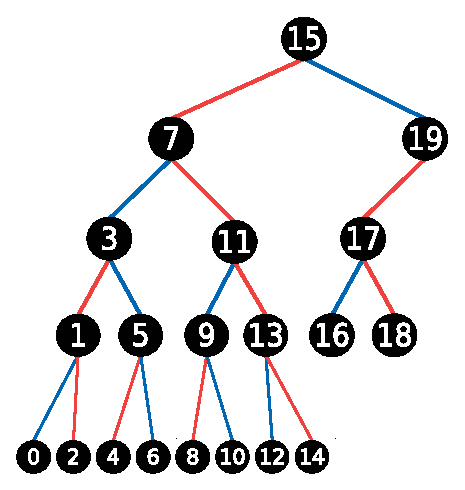
\includegraphics[scale=0.4]{images/unbalanced-S-T1-gap.eps} 
%\caption{$T_1$ in TwoTreeS}
%\label{fig:ST1}
%\end{subfigure}%
%\hfill
%\begin{subfigure}{0.49\textwidth}
%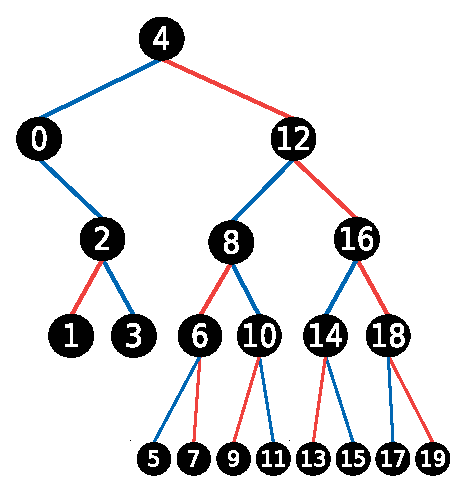
\includegraphics[scale=0.4]{images/unbalanced-S-T2-gap.eps}
%\caption{$T_2$ in TwoTreeS}
%\label{fig:ST2}
%\end{subfigure}
% 
%\caption{TwoTreeS \cite{sanders_two-tree_2009} two trees}
%\label{fig:twoTreeS}
%\end{figure}

\begin{figure}[t]
 
\begin{tabular}{cc}
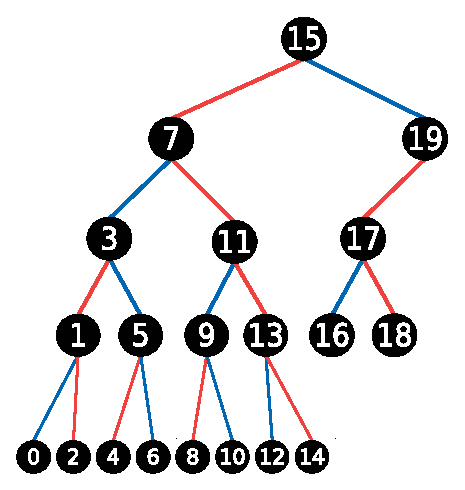
\includegraphics[scale=0.47]{images/unbalanced-S-T1-gap.eps}  & \hspace{0.4cm} 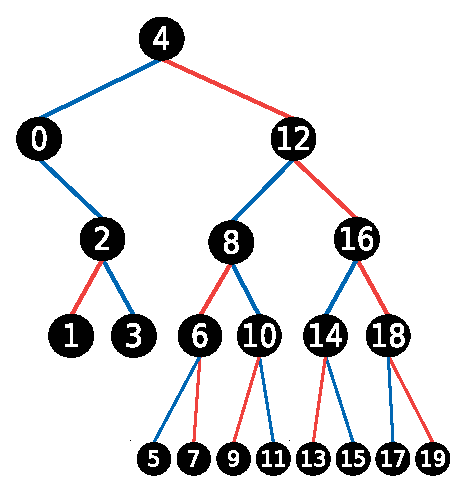
\includegraphics[scale=0.47]{images/unbalanced-S-T2-gap.eps} \\ \\
(a) $T_1$ & (b) $T_2$ \\
\end{tabular}
\caption{Design of two trees in TwoTreeS \cite{sanders_two-tree_2009} for $20$ processes}
\label{fig:twoTreeS}
\end{figure}

% \begin{figure}[h] \centering \includegraphics[width=0.5\textwidth]{images/twoTreeC.eps} \caption{\label{fig:twoTrees}} \end{figure}

%\section{TwoTreeComplete}\label{sec:TwoTreeComplete}
%As discussed in the section\ref{sec:Motivation} the sanders implementation of the tree has some disadvantage, so on the basis of those shortcomings we have proposed a simpler yet better implementation of the two tree algorithm. The idea is same which is to use two binary trees with nodes in one nodes as inner nodes in other, the difference lies in the way these trees are constructed. As the name suggests the binary tree we have created are complete binary trees, the design is simple and we have used no explicit synchronization. How the topology is to be constructed how we have calculated the number of chunks for different parameters is what we aare going to discuss in these subsections.

\section{Two Tree Complete (TwoTreeC)}\label{sec:TwoTreeC}
The idea behind TwoTreeC is rather very simple. We construct two complete binary trees $T_1$ and $T_2$ each using $P$ processes. In a rooted collective, these two trees are then assigned as left and right sub-tree of the root process. $T_1$ and $T_2$ are constructed as follows:
\begin{description}
    \item[$\bullet$]The trees are designed in such a way that leaf nodes in one tree are the inner nodes in the other and vice-versa.
    \item[$\bullet$]$T_1$(left tree) is numbered level wise, left to right, with increasing process id's starting from $0$.
    \item[$\bullet$]$T_2$(right tree) is numbered level wise, left to right, with decreasing process id's starting from $P-1$.
\end{description}
Here $P$ is the total number of processes. An example $T_1$ and $T_2$ for $20$ processes using TwoTreeC is shown in figure \ref{fig:twoTreeC}. Each process independently uses Algorithm \ref{alg:TwoTreeComp} to compute its parent and children in $T_1$ and $T_2$. With the exception of the root process, the remaining processes appear in both left and right trees. Therefore, $leftParent$ is used to denote parent of current process in left tree, and $rightParent$ is the parent of current process in right tree. $leftChild[]$ and $rightChild[]$ similarly denote the children of current node in left and right tree respectively. 

%rough explanation for nonzero root
% \begin{figure}[h]
% 
%\begin{subfigure}{0.5\textwidth}
%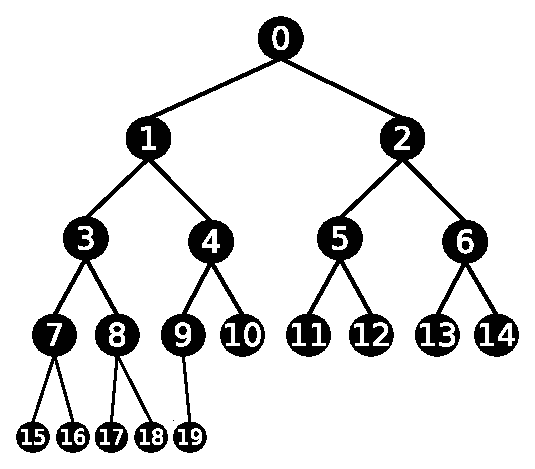
\includegraphics[width=0.5\linewidth, height=4cm]{images/complete-T1-gap.eps} 
%\caption{Caption1}
%\label{fig:CT1}
%\end{subfigure}
%\begin{subfigure}{0.5\textwidth}
%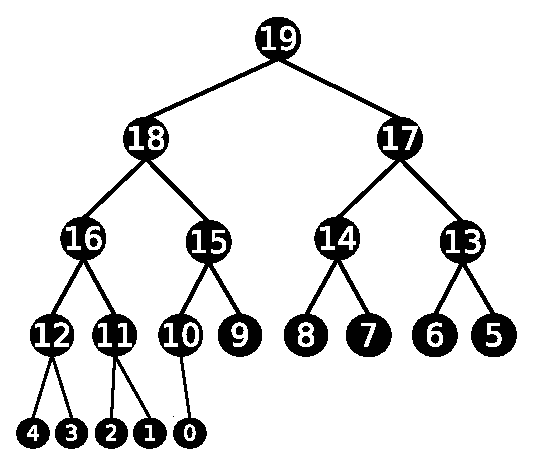
\includegraphics[width=0.5\linewidth, height=4cm]{images/complete-T2-gap.eps}
%\caption{Caption 2}
%\label{fig:CT2}
%\end{subfigure}
% 
%\caption{Caption for this figure with two images}
%\label{fig:twoTreeC}
%\end{figure}

\begin{figure}[t]
 
\begin{tabular}{cc}
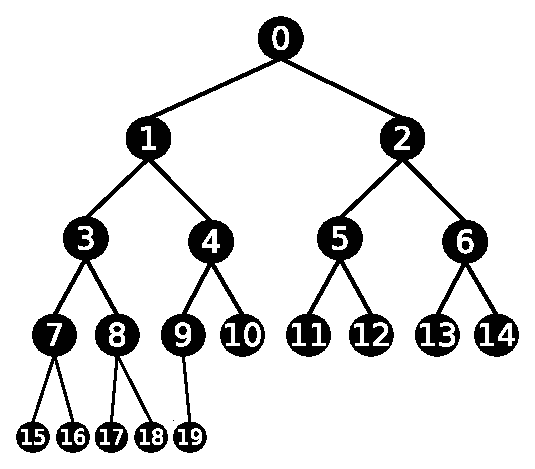
\includegraphics[scale=0.46]{images/complete-T1-gap.eps} &  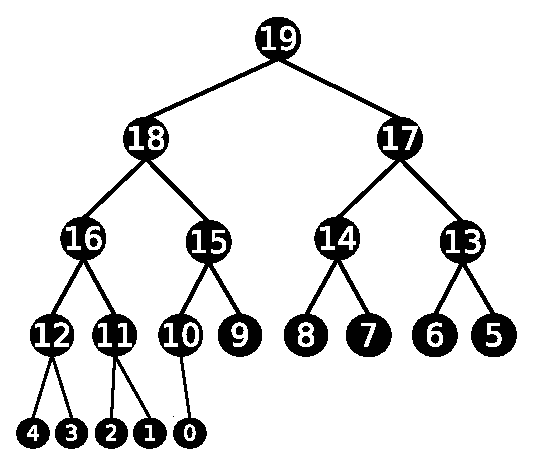
\includegraphics[scale=0.46]{images/complete-T2-gap.eps} \\ \\
(a) $T_1$ & (b) $T_2$ \\
\end{tabular}
\caption{Design of two trees in TwoTreeC for $20$ processes}
\label{fig:twoTreeC}
\end{figure}

%\begin{figure}[h] \centering \includegraphics[width=0.5\textwidth]{images/twoTreeC.eps} \caption{\label{fig:twoTrees}} \end{figure}

\begin{algorithm}
\algsetup{linenosize=\tiny}
 \scriptsize
\caption{Two Tree Complete Construction}\label{alg:TwoTreeComp}
\begin{algorithmic}[1]
\REQUIRE Number of processes $\leftarrow$ \(p\), rank $\leftarrow processId$ 
\IF{$rank$ = 0}
    \STATE numberOfLeftChildren $ \leftarrow 1$
    \STATE numberOfRightChildren $ \leftarrow 1$
    \STATE leftChild$[0] \leftarrow 1$
    \STATE rightChild$[0] \leftarrow p-1$
\ELSE[$rank \neq 0$]
    \STATE leftParent $ \leftarrow rank / 2$
    \STATE rightParent $ \leftarrow \big(p-\dfrac{p-rank}{2}\big)\%p$
    \IF{$(2 \times rank) < p$}
         \STATE numberOfLeftChildren $ \leftarrow 1$
         \STATE leftChild[0]$ \leftarrow 2 \times rank$
    \ENDIF
    \IF{$\big((2 \times rank) + 1\big) < p$}
         \STATE numberOfLeftChildren $ \leftarrow 2$
         \STATE leftChild[1]$ \leftarrow \big((2 \times rank) + 1\big)$
    \ENDIF
    \IF{$\big((2 \times rank) - p\big) > 0$}
         \STATE numberOfRightChildren $ \leftarrow 1$
         \STATE rightChild$[0] \leftarrow \big((2 \times rank) - p\big)$
    \ENDIF
    \IF{$\big((2 \times rank) - p - 1\big) > 0$}
         \STATE numberOfRightChildren $ \leftarrow 2$
         \STATE rightChild$[1] \leftarrow \big((2 \times rank) - p - 1\big)$
    \ENDIF
\ENDIF
\end{algorithmic}
\end{algorithm}

TwoTreeC implementation addresses all the observed issues with TwoTreeS. There is no overhead due to colouring or synchronization, because we perform no explicit/implicit synchronization. The construction of trees takes only O(1) time on each process.
%Throughout all of the implementation, all the send and receive operations used are non-blocking.
%Both the trees are relatively balanced than TwoTreeS. The impact of balancing has been seen in performance gain of reduce and allreduce collectives since, the communication begins at the leaf nodes in both of the collectives.

\section{Collectives with TwoTreeC}\label{sec:Operations}
The TwoTreeC topology discussed above is used to implement broadcast, reduce and allreduce operations. The broadcast and reduce operations are rooted collectives i.e., the data is either distributed by the root process (ex., broadcast) or is collected at the root process (as in reduce). We implement allreduce as a combination of broadcast and reduce collectives. Similar to binary pipeline algorithm, TwoTreeC divides message into smaller chunks and communicate the chunks in a pipeline. We describe the approaches used to calculate number of chunks for various collectives in section \ref{sec:Chunks}.  Figure \ref{fig:towtreeC_coll} depicts our basic approach to perform these collectives using TwoTreeC. Assuming the entire message is divided into $m$ small chunks, in broadcast, even numbered chunks are sent to tree $T_1$ one after the other in a pipeline. Similarly, odd numbered chunks are sent to sub-tree $T_2$. The chunks travel from leaf processes to the root in the reduce collective. Whereas, in allreduce, reduce of the entire message happens at the root process which is followed by the pipelined broadcast. More details about each of the collectives is presented below.

%\ifcmts \{\textcolor{blue}{todo @Mohit LogGP analysis for each of these approaches.}\}

\begin{figure}[h]
 
\begin{tabular}{cc}
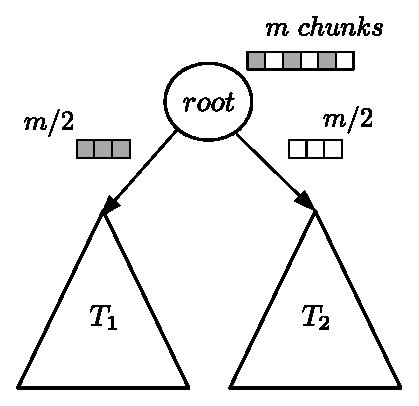
\includegraphics[scale=0.46]{images/ttbroad.eps} &  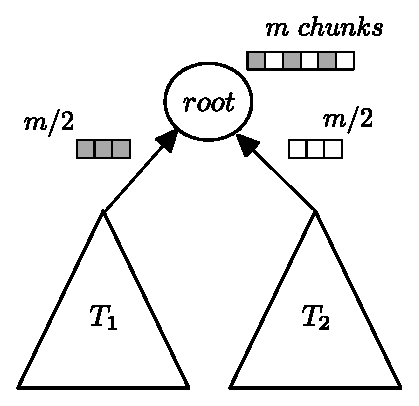
\includegraphics[scale=0.46]{images/ttreduce.eps} \\ \\
(a) Broadcast & (b) Reduce \\
\end{tabular}
\caption{Broadcast and reduce with TwoTreeC}
\label{fig:towtreeC_coll}
\end{figure}

\subsection{Broadcast} \label{sec:broad}
In broadcast collective, a message from the root process is received at all other processes in the communicator. In case rank $0$ is the root process of the collective then each process execute algorithm \ref{alg:TwoTreeComp} to find its parent and children in tree $T_1$ and $T_2$. All other processes other than the root process are available in both $T_1$ and $T_2$. Later, processes perform send and receive operations using algorithm \ref{alg:broadcastImpl}. In case the root of a rooted collective is not the process ranked $0$ but some other process $k$, then each process assumes a false rank $abs(rank-k)\%P$ and finds the false ranks of its parents and children using algorithm \ref{alg:TwoTreeComp}. These false ranks are translated back to original ranks using the same modulo function. 

The root node divides its data into a number of equal sized chunks, then one by one sends each odd-numbered chunk to the root of $T_2$ (right subtree) and each even-numbered chunk to the root of $T_1$ (left subtree). Non-root processes expect odd numbered chunks from $leftParent$ and upon receiving, forward them to their $leftChild[0]$ and $leftChild[1]$. Same task is performed in the right subtree. In the end, each process has received all the chunks, odd ones in the right tree and even ones in the left subtree.

\begin{algorithm}
\algsetup{linenosize=\tiny}
  \scriptsize
\caption{Two Tree Broadcast operation}\label{alg:broadcastImpl}
\begin{algorithmic}[1]
\REQUIRE rank $\leftarrow processId$ 
\IF{$rank$ = root}
    \FORALL{Chunks}
        \IF{Even Chunk} 
            \STATE Non-blocking send this chunk to leftChild[0]
        \ELSE
            \STATE Non-blocking send this chunk to rightChild[0]
        \ENDIF
    \ENDFOR
\ELSE[$rank \neq root$]
    \FORALL{Chunks}
        \IF{Even Chunk} 
            \STATE Non-blocking receive this chunk from leftParent
        \ELSE[Odd Chunk]
            \STATE Non-blocking receive this chunk from rightParent
        \ENDIF
    \ENDFOR
    \WHILE{all chunks not received}
        \STATE Wait until any of the receives finishes
        \IF{Even chunk received}
            \STATE Non-blocking send this chunk to leftChild[0] and leftChild[1]
        \ELSE[Odd chunk received]
            \STATE Non-blocking send this chunk to rightChild[0] and rightChild[1]
        \ENDIF
    \ENDWHILE
\ENDIF
\STATE Wait on all sends to finish
\end{algorithmic}
\end{algorithm}

\subsection{Reduce}
We use TwoTreeC to implement commutative and associative reduce collective. In reduce collective as well, we use the similar process as described in section \ref{sec:broad} for broadcast to design two trees $T_1$ and $T_2$. Similarly, $T_1$ is placed as the left subtree of the root of the collective and  $T_2$ as the right subtree. The leaf nodes begins the reduce operation by sending chunks of messages to the parent nodes as depicted in figure \ref{fig:towtreeC_coll}(b). Each non-leaf node receives the chunk number say $m$ from the child nodes and then perform the reduce operation together with its own $m^{th}$ chunk. The reduced chunk is then forwarded to the parent node and eventually reaches the root of the tree. 

\subsection{Allreduce}
We have implemented allreduce operation by doing reduce of all the chunks at the root node and then doing a broadcast. We assume process with rank $0$ to be our root process. The trees $T_1$ and $T_2$ are designed as already explained in section \ref{sec:broad}. Both of these trees are used to perform pipelined reduce operation. As soon as the root process receives any of the reduced chunk, it performs the broadcast using the same $T_1$ and $T_2$ (refer Figure \ref{fig:towtreeC_allreduce}). By doing this overlap of reduce and broadcast operations, we further improve time efficiency of our implementation as compared to first wait for all the chunks to be reduced at the root process and then beginning to broadcast. 

\begin{figure}[t]
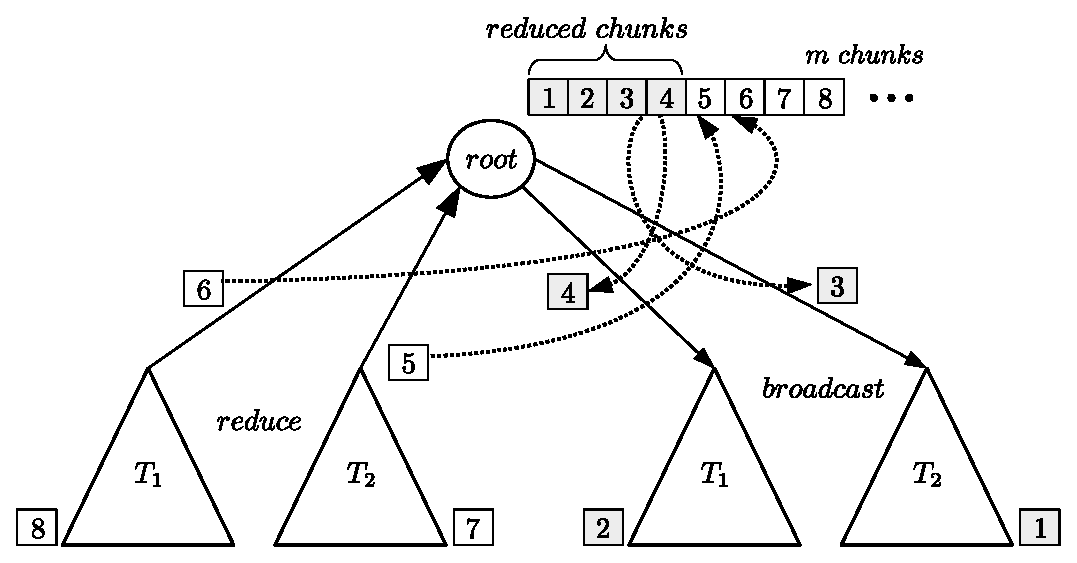
\includegraphics[scale=0.46]{images/ttallreduce.eps} \\ 
\caption{Allreduce with TwoTreeC showing overlap of reduce and broadcast}
\label{fig:towtreeC_allreduce}
\end{figure}

As can be seen in figure \ref{fig:towtreeC_allreduce}, to implement allreduce collective, two pairs of two-trees have been used. Instead of using the same pair of $T_1$ and $T_2$ for both reduce and broadcast, different pairs can also be used to further improve the time efficiency. We have designed and tested two variations of our original TwoTreeC allreduce implementation which uses different pairs for reduce and broadcast phases. 


\subsubsection{TwoTreeC+C}
The main idea behind TwoTreeC+C allreduce implementation is to improve the bandwidth utilization of the leaf nodes in the reduce phase of TwoTreeC. We design a new pair of two trees for broadcast phase (referred as $T_3$ and $T_4$) such that the nodes finishing the reduce part first in $T_1$ are closer to the root node in $T_3$ and $T_4$. The two trees for reduce phase in TwoTreeC+C is same as that of $T_1$ and $T_2$ in TwoTreeC. We have designed $T_3$ and $T_4$ (complete trees) for broadcast phase of TwoTreeC+C as follows:

\begin{description}
     \item[$\bullet$]T$_{3}$ is numbered in level wise, in increasing order (circular in range $1...P-1$) starting from $\left \lceil{\dfrac{P}{2}}\right \rceil$
     \item[$\bullet$] T$_{4}$ is numbered in level wise, in decreasing order (circular in range $1...P-1$) starting from $\left \lfloor{\dfrac{P}{2}}\right\rfloor $
 \end{description}
Figure \ref{fig:reordered} shows $T_3$ and $T_4$ for TwoTreeC+C for 20 processes.

\begin{figure}[b]
\begin{tabular}{cc}
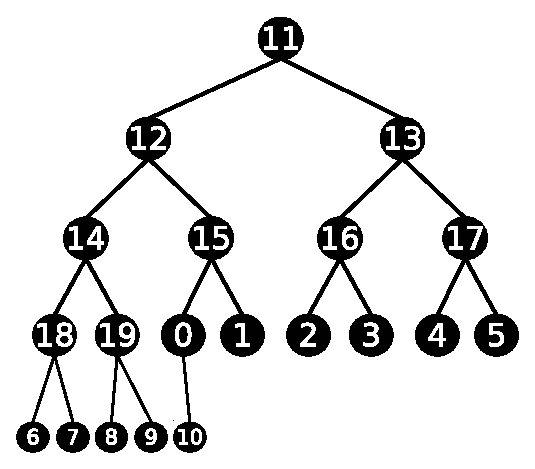
\includegraphics[scale=0.46]{images/reordered-twoTreeC-T1.eps} &  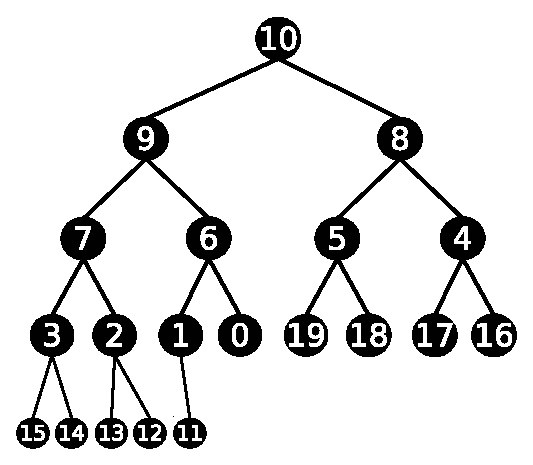
\includegraphics[scale=0.46]{images/reordered-twoTreeC-T2.eps} \\ \\
(a) $T_3$ & (b) $T_4$ \\
\end{tabular}
\caption{$T_3$ and $T_4$ for TwoTreeC+C for 20 processes}
\label{fig:reordered}
\end{figure}

%
%\begin{algorithm}[htp]
%\algsetup{linenosize=\tiny}
%\scriptsize
%\caption{Reordered Two Tree Complete Construction}\label{alg:ReorderedTwoTree}
%\SetAlgoLined\DontPrintSemicolon
%\SetKwFunction{FUNCRP}{FUNCRP}
%\SetKwFunction{FUNCONE}{FUNCONE}
%\SetKwFunction{FUNCTWO}{FUNCTWO}
%\SetKwFunction{algo}{algo}
%\SetKwProg{myproc}{Procedure}{}{}
%\SetKwProg{myalg}{Algorithm}{}{}
%
%\myproc{\FUNCRP{var}}{
%    \begin{algorithmic}[1]
%        \IF{$var = 0$}
%            \RETURN $0$
%        \ELSE
%            \RETURN $ \big(p - \dfrac{p-var}{2}\big)\%p $
%        \ENDIF
%    \end{algorithmic}
%}
%\myproc{\FUNCONE{var}}{
%    \begin{algorithmic}[1]
%        \IF{$var = 0$}
%            \RETURN $0$
%        \ELSE
%            \RETURN $ \bigg(\Big(\big((var-1-(\dfrac{p-1}{2}))+(p-1)\big) \% \big(p-1\big)\Big) + 1\bigg) $
%        \ENDIF
%    \end{algorithmic}
%}
%\myproc{\FUNCTWO{var}}{
%    \begin{algorithmic}[1]
%        \IF{$var = 0$}
%            \RETURN $0$
%        \ELSE
%            \RETURN $ \bigg(\Big(\big((var-1+(\dfrac{p-1}{2}))+(p-1)\big) \% \big(p-1\big)\Big) + 1\bigg); $
%        \ENDIF
%    \end{algorithmic}
%}
%\myalg{\algo{}} {
%\begin{algorithmic}[1]
%\REQUIRE Number of Process $\leftarrow$ \(p\), rank $\leftarrow processId$ 
%\IF{$rank$ = 0}
%    \STATE number\_leftChildren $ \leftarrow 1$
%    \STATE number\_rightChildren $ \leftarrow 1$
%    \STATE leftChild$[0] \leftarrow$ FUNCTWO($1$)
%    \STATE rightChild$[0] \leftarrow$ FUNCONE($p-1$)
%\ELSE[$rank \neq 0$]
%    \STATE leftParent $ \leftarrow$ FUNCTWO\big( FUNCONE($rank$) $ / 2$\big)
%    \STATE rightParent $ \leftarrow$ FUNCONE\Big( FUNCRP\big( FUNCTWO($rank$) \big) \Big)
%    \IF{$2 \times$ FUNCONE($rank$) $< p$}
%         \STATE number\_leftChildren $ \leftarrow 1$
%         \STATE leftChild[0]$ \leftarrow$ FUNCTWO\big( $2 \times $FUNCONE($rank$) \big)
%    \ENDIF
%    \IF{$\big(2 \times$ FUNCONE($rank$)\big)$+1 < p$}
%         \STATE number\_leftChildren $ \leftarrow 2$
%         \STATE leftChild[1]$ \leftarrow$ FUNCTWO\Big( \big($2 \times$ FUNCONE( $rank$ )\big)$+1$\Big)
%    \ENDIF
%    \IF{$\big(2 \times$ FUNCTWO($rank$)\big)$ - p > 0$}
%         \STATE number\_rightChildren $ \leftarrow 1$
%         \STATE rightChild$[0] \leftarrow$ FUNCONE\Big( \big($2 \times$ FUNCTWO( $rank$ )\big)$ - p$\Big)
%    \ENDIF
%    \IF{$\big(2 \times$ FUNCTWO($rank$)\big)$-p-1 > 0$}
%         \STATE number\_rightChildren $ \leftarrow 2$
%         \STATE rightChild$[1] \leftarrow$ FUNCONE\Big( \big($2 \times$ FUNCTWO( $rank$ )\big)$-p-1$\Big)
%    \ENDIF
%\ENDIF
%\end{algorithmic}}
%\end{algorithm}

\subsubsection{TwoTreeC+S}
As seen in the previous optimization, all-reduce operation can be improved using different algorithms for the sub parts reduce and broadcast. So similarly here this version of all-reduce operation uses the TwoTreeS for the first part $i.e.$ reduce and uses the TwoTreeC for the second part $i.e.$ broadcast.

\section{Calculation of Number of Chunks} \label{sec:Chunks}
Since the algorithms are pipelined, it is important to calculate the optimal number of chunks to divide the message into. The number of chunks and hence the size of each chunk are important factors affecting runtime. %Calculating the chunks value for different algorithms and for different parameters was also very challenging. 
We have used several methods to calculate the optimal values of the chunks for each algorithm and different number of processes.
\subsection{Mathematical Approach}
In the initial phase of the research when work was mostly concentrated on the broadcast operation, number of chunks was calculated using a mathematical expression for the run time of the algorithm and by minimizing the run time. This worked well for simple enough implementations.
\subsection{Simulation Tool}
Later on as progress was made on different implementations, as well as other operations, it gets complicated. We switched our mode of calculating chunks to using a simulator LogGOPSim, a fast simulation framework for parallel algorithms at large-scale for calculating the optimal number of chunks. The simulator gave a good idea about the behaviour of our algorithms on changing the number of chunks which was very helpful in making many further optimizations.
\subsection{Experimentation}
The results of the simulator were not always similar to the actual experimentation. A better approach was needed. Finally, instead of using one method, we use results from both the methods and also add some more random values\((\pm10\%, \pm20\%)\) so as to cover a larger range and then choose the best out of them for different number of processes and message sizes. This way we ensure that the values we used are much closer to the best values.

\section{Experimental Configuration and Parameters}\label{sec:Config}


\ifcmts \{\textcolor{blue}{todo @Mohit LogGP parameter values, other details like single process per node, etc.}\}

\section{Results}\label{sec:Results}
Mention and briefly explain all the implementations compared: linear pipeline, pipelined binary tree, our pipelined two tree, mpi standard library, scatter-gather. Conclude how our approach outperformes the rest on larger data sizes.

\ifcmts \{\textcolor{blue}{todo @Mohit plots}\}

\subsection{Broadcast}

Message Sizes : 256KB, 512KB, 1MB, 3MB, 5MB, 7MB


\begin{figure}
\centering
\begin{subfigure}{.25\textwidth}
  \centering
  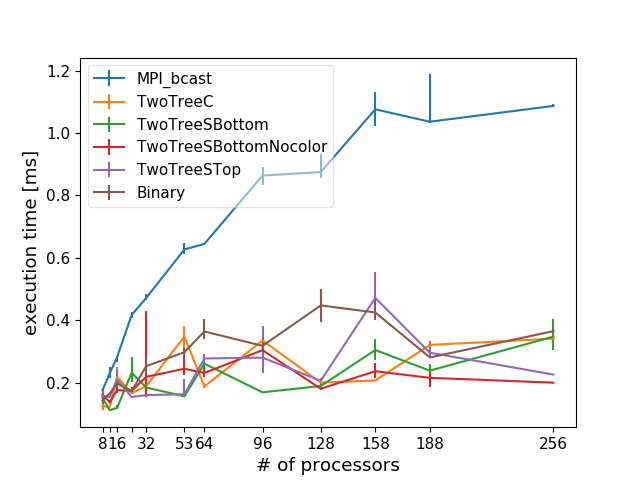
\includegraphics[width=1\linewidth]{images/Results/bcastFinal_262144B.png}
  \caption{Broadcast-256KB}
  \label{bcast-selected-256B}
\end{subfigure}%
\begin{subfigure}{.25\textwidth}
  \centering
  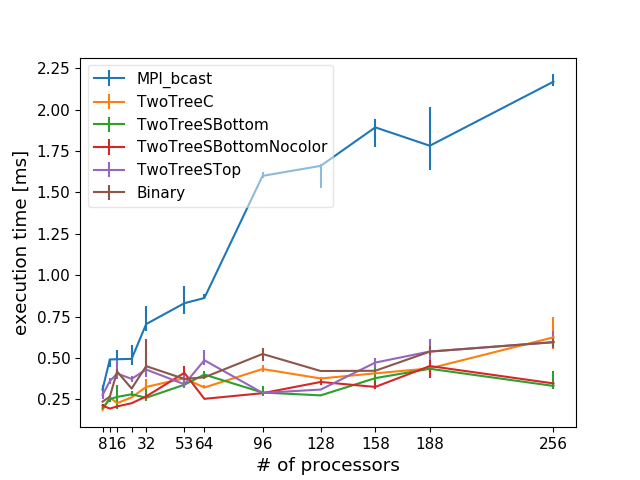
\includegraphics[width=1\linewidth]{images/Results/bcastFinal_524288B.png}
  \caption{Broadcast-512KB}
  \label{bcast-selected-512B}
\end{subfigure}
\caption{Broadcast results for small sized messages}
\label{graph-bcast-small-selected}
\end{figure}

\begin{figure}
\centering
\begin{subfigure}{.25\textwidth}
  \centering
  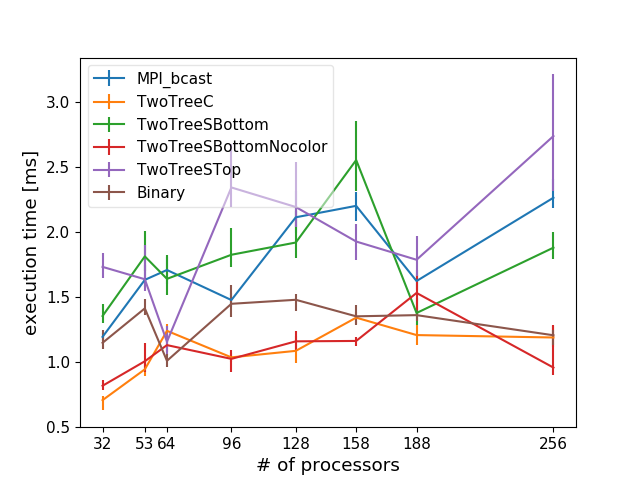
\includegraphics[width=1\linewidth]{images/Results/bcastFinal_1048576B.png}
  \caption{Broadcast-1MB}
  \label{bcast-selected-3MB}
\end{subfigure}%
\begin{subfigure}{.25\textwidth}
  \centering
  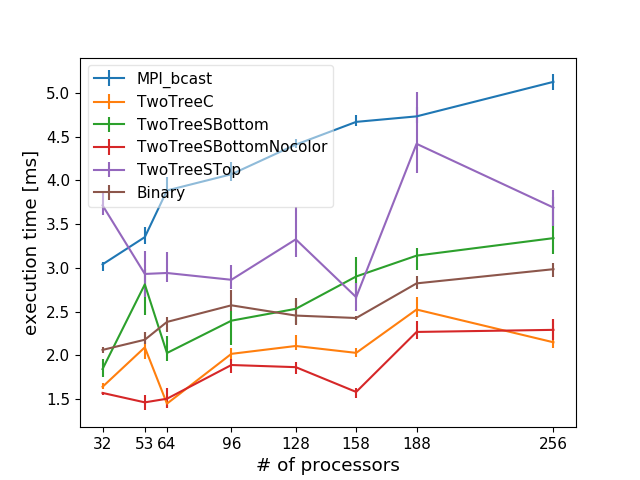
\includegraphics[width=1\linewidth]{images/Results/bcastFinal_3145728B.png}
  \caption{Broadcast-3MB}
  \label{bcast-selected-3MB}
\end{subfigure}
\caption{Broadcast results for medium sized messages}
\label{graph-bcast-medium1-selected}
\end{figure}

\begin{figure}
\centering
\begin{subfigure}{.25\textwidth}
  \centering
  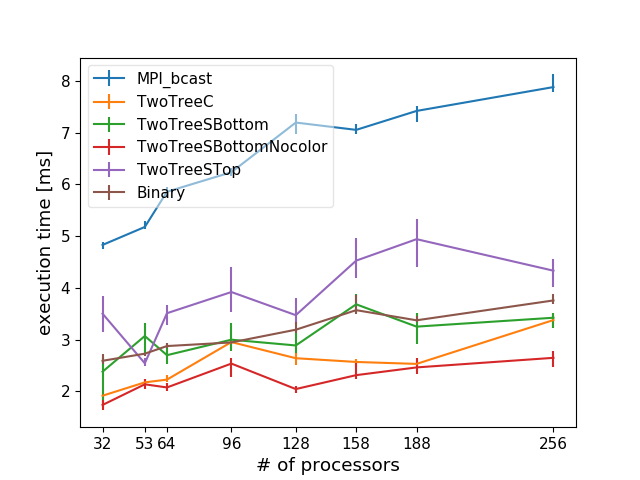
\includegraphics[width=1\linewidth]{images/Results/bcastFinal_5242880B.png}
  \caption{Broadcast-5MB}
  \label{bcast-selected-5MB}
\end{subfigure}%
\begin{subfigure}{.25\textwidth}
  \centering
  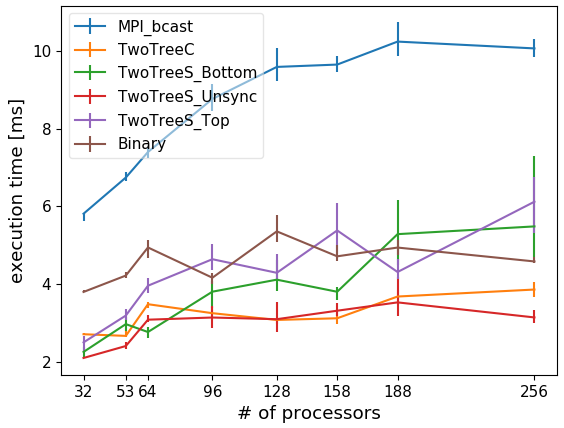
\includegraphics[width=1\linewidth]{images/Results/bcastFinal_7340032B.png}
  \caption{Broadcast-7MB}
  \label{bcast-selected-7MB}
\end{subfigure}
\caption{Broadcast results for medium sized messages}
\label{graph-bcast-medium2-selected}
\end{figure}



\subsection{Reduce}

Message Sizes : 256KB, 512KB, 1MB, 3MB, 5MB, 7MB

\begin{figure}
\centering
\begin{subfigure}{.25\textwidth}
  \centering
  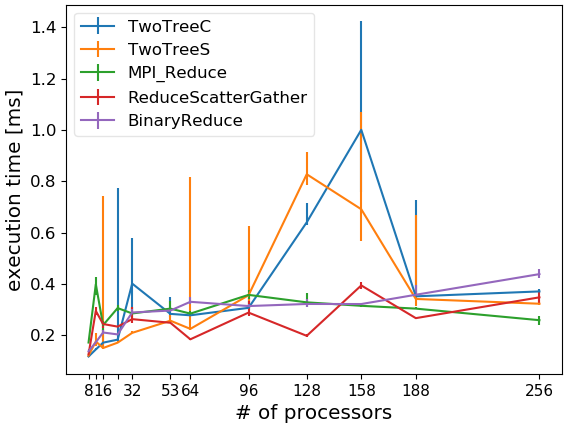
\includegraphics[width=1\linewidth]{images/Results/reducefinal_262144B.png}
  \caption{Reduce - 256KB}
  \label{reduce-selected-256B}
\end{subfigure}%
\begin{subfigure}{.25\textwidth}
  \centering
  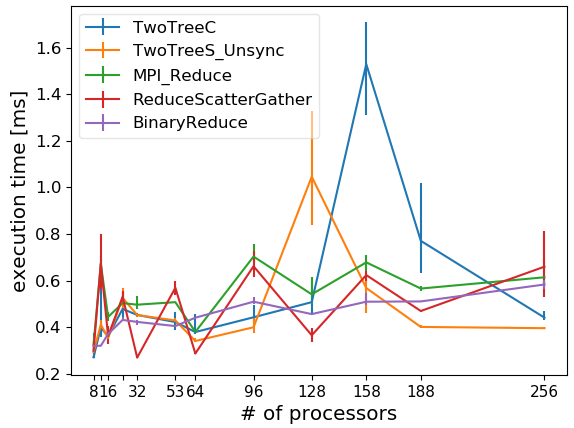
\includegraphics[width=1\linewidth]{images/Results/reducefinal_524288B.png}
  \caption{Reduce - 512KB}
  \label{reduce-selected-512B}
\end{subfigure}
\caption{Reduce results for small sized messages}
\label{graph-reduce-small-selected}
\end{figure}

\begin{figure}
\centering
\begin{subfigure}{.25\textwidth}
  \centering
  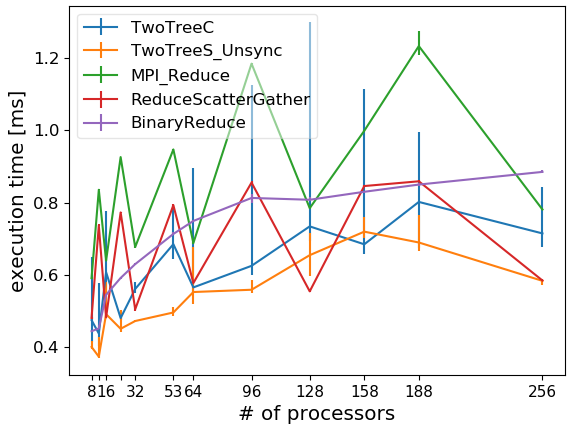
\includegraphics[width=1\linewidth]{images/Results/reducefinal_1048576B.png}
  \caption{Reduce - 1MB}
  \label{reduce-selected-1MB}
\end{subfigure}%
\begin{subfigure}{.25\textwidth}
  \centering
  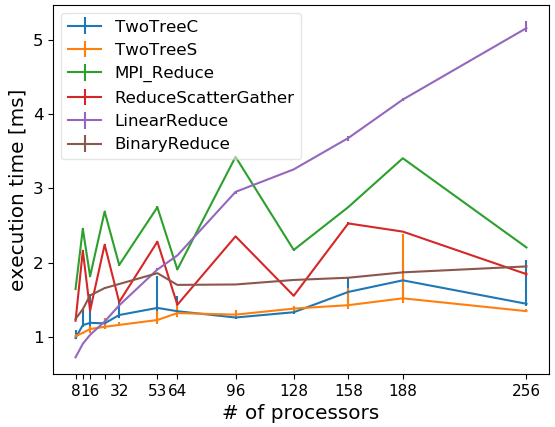
\includegraphics[width=1\linewidth]{images/Results/reducefinallinear_3145728B.png}
  \caption{Reduce - 3MB}
  \label{reduce-selected-3MB}
\end{subfigure}
\caption{Reduce results for medium sized messages}
\label{graph-reduce-medium1-selected}
\end{figure}

\begin{figure}
\centering
\begin{subfigure}{.25\textwidth}
  \centering
  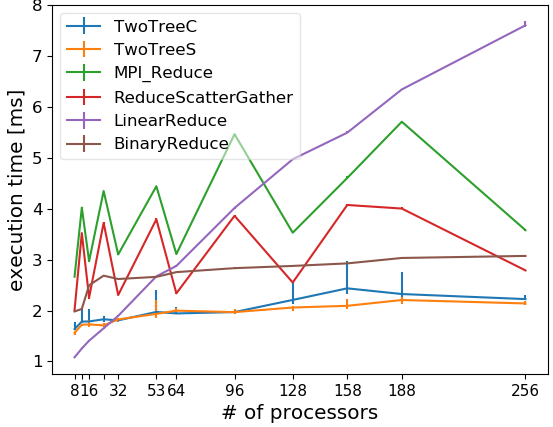
\includegraphics[width=1\linewidth]{images/Results/reducefinallinear_5242880B.png}
  \caption{Reduce - 5MB}
  \label{reduce-selected-5MB}
\end{subfigure}%
\begin{subfigure}{.25\textwidth}
  \centering
  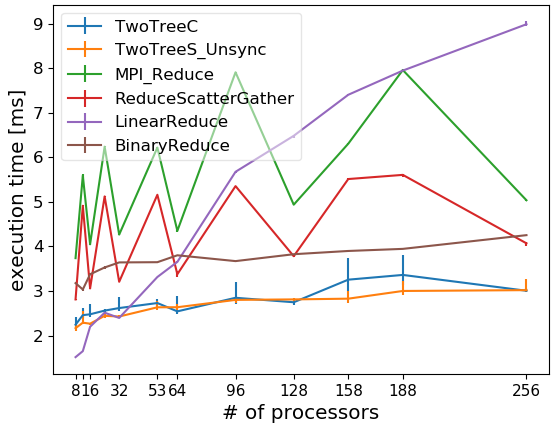
\includegraphics[width=1\linewidth]{images/Results/reducefinallinear_7340032B.png}
  \caption{Reduce - 7MB}
  \label{reduce-selected-7MB}
\end{subfigure}
\caption{Reduce results for medium sized messages}
\label{graph-reduce-medium2-selected}
\end{figure}

\subsection{All-Reduce}
\ifcmts \{\textcolor{red}{todo @Sir lower bound}\}
\begin{figure}
\centering
\begin{subfigure}{.25\textwidth}
  \centering
  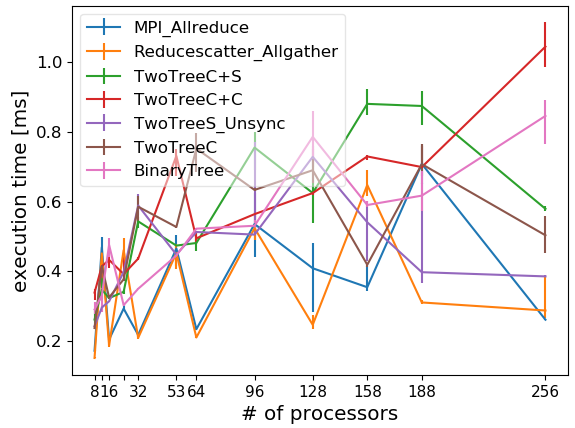
\includegraphics[width=1\linewidth]{images/Results/AllReduce/allreducecomp3_262144B.png}
  \caption{All-Reduce - 256KB}
  \label{reduce-selected-256B}
\end{subfigure}%
\begin{subfigure}{.25\textwidth}
  \centering
  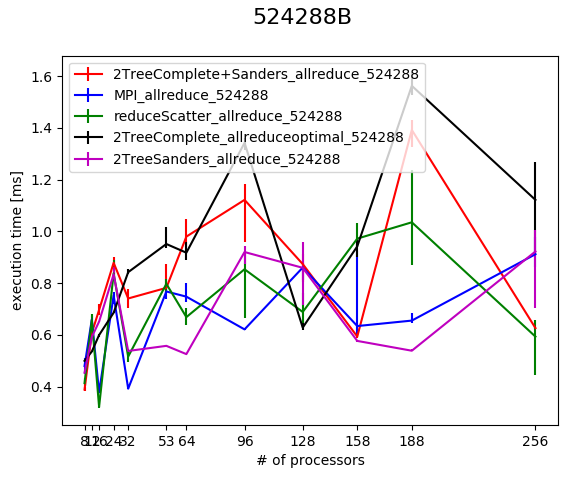
\includegraphics[width=1\linewidth]{images/Results/AllReduce/allreducecomp3_524288B.png}
  \caption{All-Reduce - 512KB}
  \label{reduce-selected-512B}
\end{subfigure}
\caption{All-Reduce results for small sized messages}
\label{graph-reduce-small-selected}
\end{figure}

\begin{figure}
\centering
\begin{subfigure}{.25\textwidth}
  \centering
  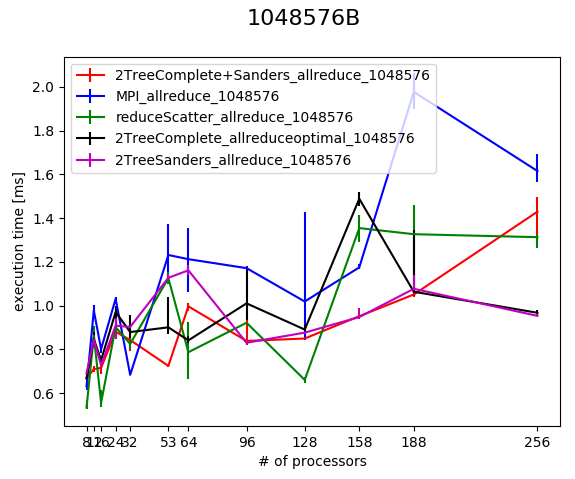
\includegraphics[width=1\linewidth]{images/Results/AllReduce/Allreduce_comp2_1048576B.png}
  \caption{All-Reduce - 1MB}
  \label{reduce-selected-1MB}
\end{subfigure}%
\begin{subfigure}{.25\textwidth}
  \centering
  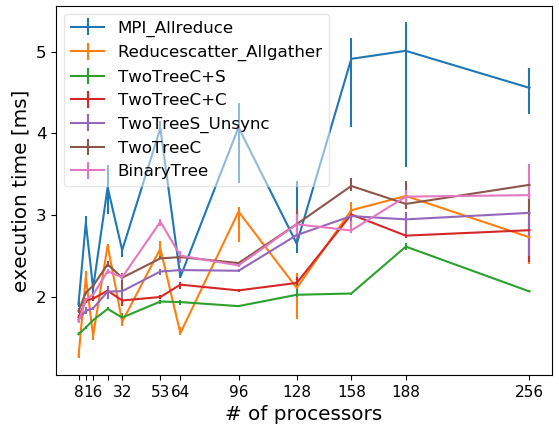
\includegraphics[width=1\linewidth]{images/Results/AllReduce/Allreduce_comp2_3145728B.png}
  \caption{All-Reduce - 3MB}
  \label{reduce-selected-3MB}
\end{subfigure}
\caption{All-Reduce results for medium sized messages}
\label{graph-reduce-medium1-selected}
\end{figure}

\begin{figure}
\centering
\begin{subfigure}{.25\textwidth}
  \centering
  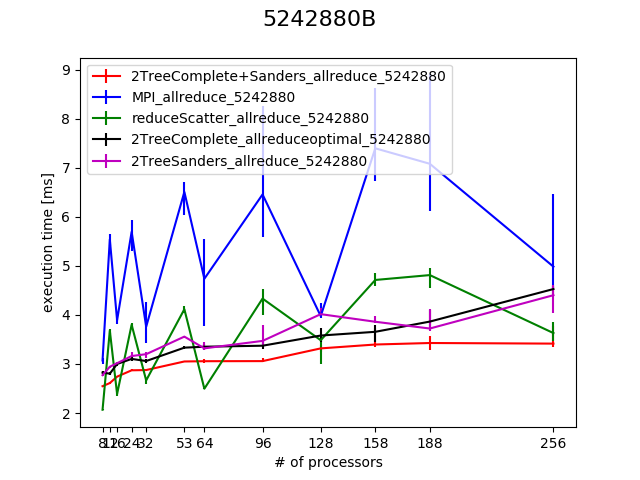
\includegraphics[width=1\linewidth]{images/Results/AllReduce/Allreduce_comp2_5242880B.png}
  \caption{All-Reduce - 5MB}
  \label{reduce-selected-5MB}
\end{subfigure}%
\begin{subfigure}{.25\textwidth}
  \centering
  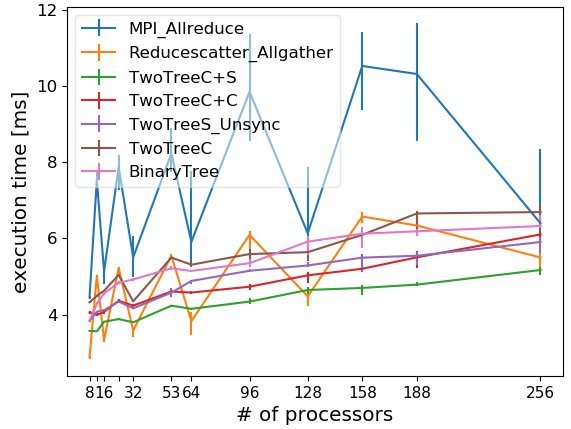
\includegraphics[width=1\linewidth]{images/Results/AllReduce/Allreduce_comp2_7340032B.png}
  \caption{All-Reduce - 7MB}
  \label{reduce-selected-7MB}
\end{subfigure}
\caption{All-Reduce results for medium sized messages}
\label{graph-reduce-medium2-selected}
\end{figure}

\begin{figure}
\centering
\begin{subfigure}{.25\textwidth}
  \centering
  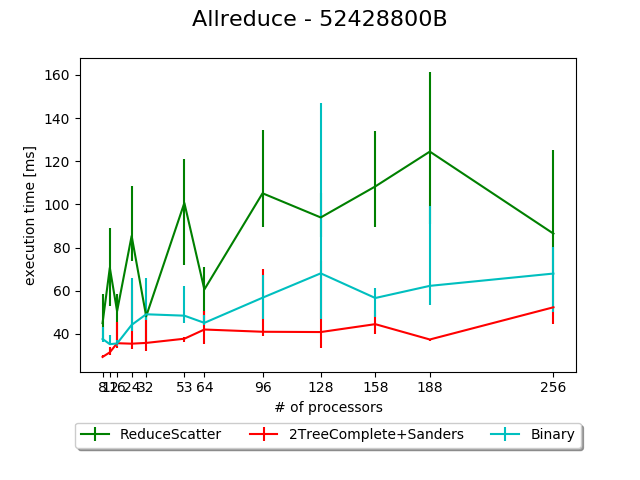
\includegraphics[width=1\linewidth]{images/Results/AllReduce/AllReduceComp2_52428800B.png}
  \caption{All-Reduce - 50MB}
  \label{reduce-selected-5MB}
\end{subfigure}%
\begin{subfigure}{.25\textwidth}
  \centering
  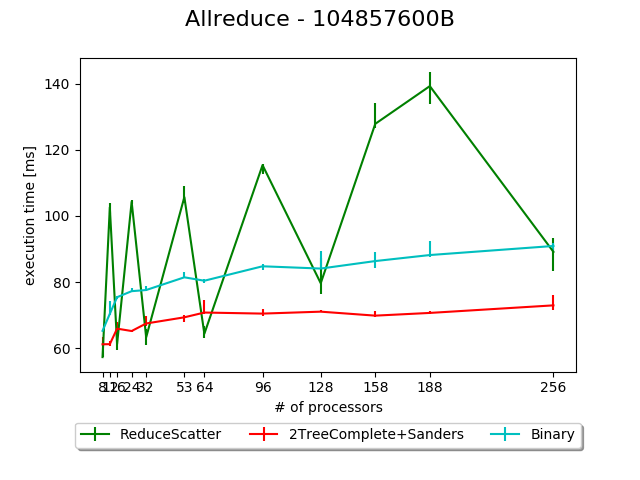
\includegraphics[width=1\linewidth]{images/Results/AllReduce/AllReduceComp2_104857600B.png}
  \caption{All-Reduce - 100MB}
  \label{reduce-selected-7MB}
\end{subfigure}
\begin{subfigure}{0.5\textwidth}
  \centering
  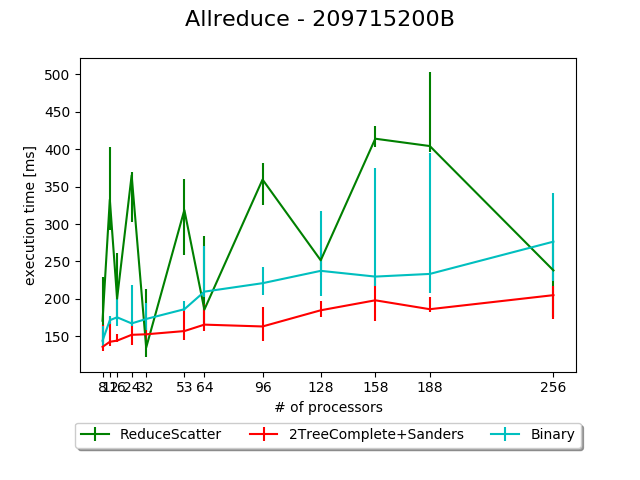
\includegraphics[width=0.5\linewidth]{images/Results/AllReduce/AllReduceComp2_209715200B.png}
  \caption{All-Reduce - 200MB}
  \label{reduce-selected-7MB}
\end{subfigure}
\caption{All-Reduce results for large sized messages}
\label{graph-reduce-medium2-selected}
\end{figure}

\subsection{Optimal Number of Chunks}

\begin{table}[t]

\caption{Broadcast - TwoTreeC}
\begin{center}
\tablefont
\begin{tabular}{|c|c|c|c|c|c|c|c|c|c|}
\hline
& \multicolumn{8}{c|}{Number of Processes} \\
\hline
Size & 32 & 53 & 64 & 96 & 128 & 158 & 188 & 256\\
\hline
 256 KB & 4 & 7 & 10 & 14 & 6 & 6 & 10 & 10\\
 512 KB & 10 & 10 & 10 & 15 & 14 & 8 & 15 & 14\\
 1 MB & 8 & 8 & 16 & 16 & 15 & 15 & 15 & 12\\
 3 MB & 27 & 27 & 24 & 27 & 27 & 16 & 25 & 24\\
 5 MB & 20 & 45 & 45 & 45 & 45 & 45 & 45 & 45\\
 7 MB & 29 & 24 & 46 & 58 & 32 & 32 & 32 & 57\\
\hline
\end{tabular}
\end{center}
\end{table}

\begin{table}[]
\caption{Reduce - TwoTreeC}
\begin{center}
\tablefont
\begin{tabular}{|c|c|c|c|c|c|c|c|c|c|c|c|c|c|}
\hline
& \multicolumn{12}{c|}{Number of Processes} \\
\hline
Size & 8 & 12 & 16 & 24 & 32 & 53 & 64 & 96 & 128 & 158 & 188 & 256\\
\hline
 256 KB & 4 & 4 & 4 & 4 & 3 & 2 & 3 & 3 & 1 & 2 & 3 & 3\\
 512 KB & 4 & 4 & 4 & 4 & 4 & 6 & 12 & 9 & 9 & 12 & 12 & 12\\
 1 MB & 4 & 12 & 4 & 12 & 6 & 9 & 12 & 12 & 8 & 12 & 12 & 17\\
 3 MB & 14 & 10 & 18 & 22 & 15 & 24 & 15 & 30 & 40 & 24 & 24 & 30\\
 5 MB & 18 & 15 & 18 & 26 & 38 & 24 & 30 & 40 & 40 & 36 & 30 & 30\\
 7 MB & 14 & 20 & 34 & 26 & 38 & 24 & 40 & 30 & 40 & 30 & 52 & 40\\
\hline
\end{tabular}
\end{center}
\end{table}

\begin{table}[]
\caption{Allreduce - TwoTreeC+S}
\begin{center}
\tablefont
\begin{tabular}{|c|c|c|c|c|c|c|c|c|c|c|c|c|}
\hline
 & \multicolumn{12}{c|}{Number of Processes} \\
\hline
 Size & 8 & 12 & 16 & 24 & 32 & 53 & 64 & 96 & 128 & 158 & 188 & 256\\
\hline
 256 KB & 2 & 2 & 2 & 2 & 2 & 2 & 2 & 2 & 2 & 2 & 2 & 2\\
 512 KB & 2 & 2 & 2 & 2 & 2 & 2 & 2 & 2 & 6 & 6 & 2 & 6\\
 1 MB & 4 & 4 & 5 & 5 & 6 & 20 & 20 & 18 & 18 & 14 & 12 & 18\\
 3 MB & 10 & 10 & 12 & 12 & 18 & 18 & 18 & 21 & 21 & 18 & 16 & 18\\
 5 MB & 12 & 12 & 14 & 14 & 18 & 18 & 18 & 20 & 21 & 16 & 24 & 18\\
 7 MB & 12 & 12 & 14 & 14 & 33 & 18 & 18 & 20 & 21 & 26 & 24 & 18\\
\hline
\end{tabular}
\end{center}
\end{table}

% Text of paper \ldots

% \section{Topologies}\label{sec:Topologies}
% Different algorithms for different operations such as BroadCast, Reduce and Allreduce uses different topologies. Topologies defines the way in which an algorithm constraints a process to be virtually connected to only a limited number of other process, i.e.\ message propagation between processes. In this section we introduce a few known and some new topologies which we will further use in our algorithms.

% \subsection{Binomial Tree}
% A binomial tree is implemented as a set of binomial trees, which are defined recursively as follows:
% \begin{description}
%     \item[$\bullet$] A binomial tree of order 0 is a single node
%     \item[$\bullet$] A binomial tree of order k has a root node whose children are roots of binomial trees of orders $k−1$, $k−2$, ..., $2$, $1$, $0$ (in this order).
% \end{description}
% Tree Construction is shown in the Algorithm \ref{alg:binomialTree}

% \begin{algorithm}
% \caption{Binomial Tree Construction}\label{alg:binomialTree}
% \begin{algorithmic}[1]
% \REQUIRE Number of Process \(p\)
% \STATE number\_childs $ \leftarrow 0$
% \STATE parent $ \leftarrow -1$
% \STATE childs $ \leftarrow$ Array of max length $p$
% \FOR{i in $0$ to $\left \lceil{(log2(p))}\right \rceil - 1$}
%     \STATE p2r $ \leftarrow 2^{r}$
%     \STATE peer $ \leftarrow rank + p2r$
%     \IF{$peer < p$ and $rank < p2r$}
%         \STATE childs$[no\_childs] \leftarrow peer$
%         \STATE number\_childs $ \pluseq 1$
%     \ENDIF
%     \STATE peer $ \leftarrow rank - p2r$
%     \IF{$rank \geq p2r$ and $rank < 2^{r+1}$}
%         \STATE parent $ \leftarrow peer$
%     \ENDIF
% \ENDFOR
% \end{algorithmic}
% \end{algorithm}


% \subsection{Binary Tree}\label{subs:BinaryTree}
% Binary Tree is a tree data structure in which each node has at most two childrens which are called Right and Left Childs and one parent node. The top node is known as the root node. There are several types of binary trees, but the one we have used is a complete binary tree. In a complete Binary Tree all levels are completely filled except possibly the last level and the last level has all keys as left as possible. This tree can be easily constructed as shown in the Algorithm \ref{alg:binaryTree}. Rank is the process Id.


% \begin{algorithm}
% \caption{Binary Tree Construction}\label{alg:binaryTree}
% \begin{algorithmic}[1]
% \REQUIRE Number of Process $\leftarrow$ \(p\), rank $\leftarrow processId$ 
% \STATE parent $ \leftarrow \dfrac{rank-1}{2}$
% \IF{$(2 \times rank) + 1 < p$}
%     \STATE number\_Children $ \leftarrow 1$
%     \STATE Child$[0]\leftarrow 2 \times rank + 1$
% \ENDIF
% \IF{$(2 \times rank) + 2 < p$}
%     \STATE number\_Children $ \leftarrow 2$
%     \STATE Child$[1] \leftarrow 2 \times rank + 2$
% \ENDIF
% \end{algorithmic}
% \end{algorithm}

% \subsection{Reverese Order Binary Tree}\label{subs:ReverseBinary}
% Reverse Order Binary Tree is similar to the binary tree(see \ref{subs:BinaryTree}) in structure, the only difference is the numbering of nodes. Unlike binary tree the numbering here is done in level wise, left to right in decreasing order. The construction of such a tree is shown in the Algorithm \ref{alg:ReverseBianry}.

% \begin{algorithm}
% \caption{Reverse Order Binary Tree Construction}\label{alg:ReverseBianry}
% \begin{algorithmic}[1]
% \REQUIRE Number of Process $\leftarrow$ \(p\), rank $\leftarrow processId$ 
% \STATE parent $ \leftarrow \Big(p - \big(\dfrac{p-rank-1}{2}\big)\Big)\%p$
% \IF{$0 < \Big(p - \big(2 \times (p-rank)\big) - 1\Big) < p$}
%     \STATE number\_Children $ \leftarrow 1$
%     \STATE Child$[0]\leftarrow \Big(p - \big(2 \times (p-rank)\big) - 1\Big)$
% \ENDIF
% \IF{$0 < \Big(p - \big(2 \times (p-rank)\big) - 2\Big) < p$}
%     \STATE number\_Children $ \leftarrow 2$
%     \STATE Child$[1] \leftarrow \Big(p - \big(2 \times (p-rank)\big) - 2\Big)$
% \ENDIF
% \end{algorithmic}
% \end{algorithm}

% \subsection{Two Tree Complete}\label{subs:TwoTreeComplete}
% Two Tree is an idea used to improve the bandwidth utilization in the binary tree. As the name suggest it consists of two complete binary trees T$_{1}$ and T$_{2}$ both constructed using $P-1$ processes, these two trees are then assigned as left and right subtree of the root node. The important part is the construction of these two trees T$_{1}$ and T$_{2}$ which is as follows:
% \begin{description}
%     \item[$\bullet$]These trees are designed in such a way that leaf nodes in one tree are the inner nodes in the other and vice-versa.
%     \item[$\bullet$]T$_{1}$ is numbered in level wise, left to right, increasing order starting form $1$.
%     \item[$\bullet$]T$_{2}$ is numbered in level wise, left to right, decreasing order starting form $P-1$.
% \end{description}
%  Here P is the total number of processes. Tree Construction is shown in Algorithm \ref{alg:TwoTreeComp}.
 
% \begin{algorithm}
% \caption{Two Tree Complete Construction}\label{alg:TwoTreeComp}
% \begin{algorithmic}[1]
% \REQUIRE Number of Process $\leftarrow$ \(p\), rank $\leftarrow processId$ 
% \IF{$rank$ = 0}
%     \STATE number\_leftChildren $ \leftarrow 1$
%     \STATE number\_rightChildren $ \leftarrow 1$
%     \STATE leftChild$[0] \leftarrow 1$
%     \STATE rightChild$[0] \leftarrow p-1$
% \ELSE[$rank \neq 0$]
%     \STATE leftParent $ \leftarrow rank / 2$
%     \STATE rightParent $ \leftarrow \big(p-\dfrac{p-rank}{2}\big)\%p$
%     \IF{$(2 \times rank) < p$}
%          \STATE number\_leftChildren $ \leftarrow 1$
%          \STATE leftChild[0]$ \leftarrow 2 \times rank$
%     \ENDIF
%     \IF{$\big((2 \times rank) + 1\big) < p$}
%          \STATE number\_leftChildren $ \leftarrow 2$
%          \STATE leftChild[1]$ \leftarrow \big((2 \times rank) + 1\big)$
%     \ENDIF
%     \IF{$\big((2 \times rank) - p\big) > 0$}
%          \STATE number\_rightChildren $ \leftarrow 1$
%          \STATE rightChild$[0] \leftarrow \big((2 \times rank) - p\big)$
%     \ENDIF
%     \IF{$\big((2 \times rank) - p - 1\big) > 0$}
%          \STATE number\_rightChildren $ \leftarrow 2$
%          \STATE rightChild$[1] \leftarrow \big((2 \times rank) - p - 1\big)$
%     \ENDIF
% \ENDIF
% \end{algorithmic}
% \end{algorithm}

% \subsection{Reordered Two Tree Complete}
% Here P is the total number of processes. It can be easily constructed as shown in Algorithm \ref{alg:ReorderedTwoTree}.

% \begin{algorithm}[htp]
% \caption{Reordered Two Tree Complete Construction}\label{alg:ReorderedTwoTree}
% \SetAlgoLined\DontPrintSemicolon
% \SetKwFunction{FUNCRP}{FUNCRP}
% \SetKwFunction{FUNCONE}{FUNCONE}
% \SetKwFunction{FUNCTWO}{FUNCTWO}
% \SetKwFunction{algo}{algo}
% \SetKwProg{myproc}{Procedure}{}{}
% \SetKwProg{myalg}{Algorithm}{}{}

% \myproc{\FUNCRP{var}}{
%     \begin{algorithmic}[1]
%         \IF{$var = 0$}
%             \RETURN $0$
%         \ELSE
%             \RETURN $ \big(p - \dfrac{p-var}{2}\big)\%p $
%         \ENDIF
%     \end{algorithmic}
% }
% \myproc{\FUNCONE{var}}{
%     \begin{algorithmic}[1]
%         \IF{$var = 0$}
%             \RETURN $0$
%         \ELSE
%             \RETURN $ \bigg(\Big(\big((var-1-(\dfrac{p-1}{2}))+(p-1)\big) \% \big(p-1\big)\Big) + 1\bigg) $
%         \ENDIF
%     \end{algorithmic}
% }
% \myproc{\FUNCTWO{var}}{
%     \begin{algorithmic}[1]
%         \IF{$var = 0$}
%             \RETURN $0$
%         \ELSE
%             \RETURN $ \bigg(\Big(\big((var-1+(\dfrac{p-1}{2}))+(p-1)\big) \% \big(p-1\big)\Big) + 1\bigg); $
%         \ENDIF
%     \end{algorithmic}
% }
% \myalg{\algo{}} {
% \begin{algorithmic}[1]
% \REQUIRE Number of Process $\leftarrow$ \(p\), rank $\leftarrow processId$ 
% \IF{$rank$ = 0}
%     \STATE number\_leftChildren $ \leftarrow 1$
%     \STATE number\_rightChildren $ \leftarrow 1$
%     \STATE leftChild$[0] \leftarrow$ FUNCTWO($1$)
%     \STATE rightChild$[0] \leftarrow$ FUNCONE($p-1$)
% \ELSE[$rank \neq 0$]
%     \STATE leftParent $ \leftarrow$ FUNCTWO\big( FUNCONE($rank$) $ / 2$\big)
%     \STATE rightParent $ \leftarrow$ FUNCONE\Big( FUNCRP\big( FUNCTWO($rank$) \big) \Big)
%     \IF{$2 \times$ FUNCONE($rank$) $< p$}
%          \STATE number\_leftChildren $ \leftarrow 1$
%          \STATE leftChild[0]$ \leftarrow$ FUNCTWO\big( $2 \times $FUNCONE($rank$) \big)
%     \ENDIF
%     \IF{$\big(2 \times$ FUNCONE($rank$)\big)$+1 < p$}
%          \STATE number\_leftChildren $ \leftarrow 2$
%          \STATE leftChild[1]$ \leftarrow$ FUNCTWO\Big( \big($2 \times$ FUNCONE( $rank$ )\big)$+1$\Big)
%     \ENDIF
%     \IF{$\big(2 \times$ FUNCTWO($rank$)\big)$ - p > 0$}
%          \STATE number\_rightChildren $ \leftarrow 1$
%          \STATE rightChild$[0] \leftarrow$ FUNCONE\Big( \big($2 \times$ FUNCTWO( $rank$ )\big)$ - p$\Big)
%     \ENDIF
%     \IF{$\big(2 \times$ FUNCTWO($rank$)\big)$-p-1 > 0$}
%          \STATE number\_rightChildren $ \leftarrow 2$
%          \STATE rightChild$[1] \leftarrow$ FUNCONE\Big( \big($2 \times$ FUNCTWO( $rank$ )\big)$-p-1$\Big)
%     \ENDIF
% \ENDIF
% \end{algorithmic}}
% \end{algorithm}

% \subsection{Linear Tree}\label{subs:LinearTree}

% \subsection{Ring Tree}\label{subs:RingTree}

% \subsection{Two Tree Sanders}\label{subs:TwoTreeSanders}


% \section{Algorithms}
% In this section we will discuss the algorithms and their different versions which we have implemented using different topologies described in the Section \ref{sec:Topologies}. 

% \section{Pipeline Algorithms}
% Pipeline Algorithms are based on the idea to divide a large message into smaller pieces and then to distribute these pieces among several processes in a pipeline fashion. Many virtual topologies can be used to implement such algorithms, we have implemented a few and will discuss them one by one here :

% \subsection{Linear Pipeline}\label{imp:LinearPipeline}
% This is the simplest of all in which we virtually arrange all process in a linear fashion, such that each process is connected to two other process except the two first and the last which are connected only to one process. The topology and the way of construction is shown in the section \ref{subs:LinearTree}. We have used this algorithm to implement the three important collective operations: BroadCast, Reduce, All-Reduce.

% \heading{BroadCast}
% % \begin{minipage}[b]{0.5\linewidth}
% BroadCast operation can be implemented using linear Pipeline in a way that each process except the first(root) receives all message chunks from its parent and every node(except the last) after receiving a chunk sends that chunk to its child node. This way the message from root node is distributed among all processes. The process topology is shown in the figure \ref{fig:LinearBroadcast}, directed arrows represents the flow of the pipeline.\newpage
% % \end{minipage}

% \begin{figure}
% \centering
% \begin{subfigure}{.2\textwidth}
%   \centering
%   \includegraphics[width=.5\linewidth]{images/sampleimg.jpg}
%   \caption{BroadCast}
%   \label{fig:LinearBroadcast}
% \end{subfigure}%
% \begin{subfigure}{.2\textwidth}
%   \centering
%   \includegraphics[width=.5\linewidth]{images/sampleimg.jpg}
%   \caption{Reduce}
%   \label{fig:LinearReduce}
% \end{subfigure}
% \caption{A figure with two subfigures}
% \label{fig:LinearAlgo}
% \end{figure}

% \heading{Reduce}
% % \begin{minipage}[b]{0.5\linewidth}
% To implement the reduce operation we can use Linear Pipeline algorithm in a way that each process except the last node receives all reduced chunks from its child node. On receiving the reduced chunk they performs the reduce operation on the received chunk and the personal message chunk. Then finally every node(except the first) sends the reduced message to its parent node. This way the root process gets the reduced message. The communication flow is shown in the figure \ref{fig:LinearReduce}.
% % \end{minipage}

% \heading{All-Reduce}
% \begin{wrapfigure}{R}{0.2\textwidth}
% \centering
% \includegraphics[width=0.5\linewidth]{images/sampleimg.jpg}
% \caption{\label{fig:frog1}This is a figure caption.}\label{fig:LinearAllReduce}
% \end{wrapfigure}
% To implement the all-reduce operation, we divide the operation in two parts. First the message is reduced to the root process and is then broadcasted to all the other nodes. These two operation are allowed to overlap. For this task, We use the ring topology for which the construction is described in \ref{subs:RingTree} . Operation is started by the last node($P-1$) and also finishes with the same node. The process is described using directed edges in the figure \ref{fig:LinearAllReduce}.

% \subsection{Binary Pipeline}\label{imp:BinaryPipeline}
% For this pipeline algorithm we use the topology in which the processes are virtually arranged in a binary fashion, which means every node is connected to three nodes, two being the child nodes and one parent node. The topology and the way of construction is shown in the section\ref{subs:BinaryTree}. We have used this algorithm to implement the three important collective operations: BroadCast, Reduce, All-Reduce.
 
% \heading{BroadCast}
% The process start with the root node by sending all chunks first to the left child then to the right child one by one, every process except the root node receives the chunks from its parents, and on receiving a chunk send it to the child nodes(if any). This way the message is broadcasted to all the processes. The topology and the flow of communication is shown in figure \ref{fig:BinaryBroadcast}.

% \begin{figure}
% \centering
% \begin{subfigure}{.2\textwidth}
%   \centering
%   \includegraphics[width=.5\linewidth]{images/sampleimg.jpg}
%   \caption{BroadCast}
%   \label{fig:BinaryBroadcast}
% \end{subfigure}%
% \begin{subfigure}{.2\textwidth}
%   \centering
%   \includegraphics[width=.5\linewidth]{images/sampleimg.jpg}
%   \caption{Reduce}
%   \label{fig:BinaryReduce}
% \end{subfigure}
% \caption{A figure with two subfigures}
% \label{fig:BinaryAlgo}
% \end{figure}

% \heading{Reduce}
% The reduce start operation start with the leaf nodes by sending the personal message chunks to the parent nodes, Each node except the leaf nodes receives the reduced message from their child nodes and then perform the reduce operation on personal message chunk and corresponding received chunks from all child nodes. Then Finally sends the reduced chunk to the parent node. The topology and the flow of communication is shown in the figure \ref{fig:BinaryReduce}.

% \heading{All-Reduce}
% \begin{wrapfigure}{R}{0.2\textwidth}
% \centering
% \includegraphics[width=0.5\linewidth]{images/sampleimg.jpg}
% \caption{\label{fig:frog1}This is a figure caption.}\label{fig:BinaryAllReduce}
% \end{wrapfigure}
% As discussed earlier all-Reduce operation can be seen as combination of two parts, Reduce and Broadcast. Since these two operations can be overlapped as we are using the pipeline algorithm, We have used two different topologies for the two operations so as to increase the overlap. For the reduce part we have used the topology described in \ref{subs:BinaryTree}, whereas for the broadCast part we have used the topology described in \ref{subs:ReverseBinary}. The advantage of using different topology for broadcast part is that this tolopgy is designed in a way that nodes far from the root in reduce part are closer in broadcast part, hence increasing the overlap. For example see figure \ref{fig:BinaryAllReduce}

% \subsection{Two Tree Pipeline}\label{imp:TwoTree}
% As we saw above in \ref{imp:BinaryPipeline} the leaf nodes in the binary tree do not use their sending bandwidth in broadcast operation and receiving bandwidth in reduce operation. To utilize the bandwidth optimally Two Tree algorithm is used. The idea is to employ two trees with different structure such that leaf nodes are different in both trees. Then divide the chunks equally to be communicated between both these trees. There are two different version of this algorithm that we have implemented for different operations.

% \subsubsection{Two Tree Sanders}
% Sanders and Traff demonstrate such a two-tree virtual topology that achieves full bandwidth, extending and simplifying an earlier algorithm . They also describe a scheduling algorithm to define from which parent node the data should be received at the current step and to which child node the data should be forwarded. The topology construction is described in \ref{subs:TwoTreeSanders}. The algorithm is scheduled using the coloring synchronization method. In order to simultaneously use both trees for collective communication the edges are virtually colored in such a way that :
% \begin{description}
%     \item[$\bullet$]No process is connected to its parent node in both trees T$_1$ and T$_2$ using the same color edges.
%     \item[$\bullet$]No process is connected to its child nodes in either T$_1$ or T$_2$ using the same color edges.
% \end{description}

% The color of the edges tells that a particular edge will be used in a particular step or not. For time step t, all the edges colored with j \% 2 are used. We have implemented this topology with the color scheduling for the broadcast operation.

% \subsubsection{Two Tree Complete}
% As we implemented and analyzed the Two Tree Sanders algorithm we came across several issues with it, and to resolve those issues we proposed a different version of Two Tree Pipeline algorithm. This version is different from Sanders version in two aspects. First is that it does not require any synchronizations and the second one is the difference in the topology. The construction methodology for this topology is shown in the algorithm \ref{alg:TwoTreeComp}. 
% The major advantage of using this algorithm and the issues with the sanders version are discussed below :
% \begin{description}
%     \item[$\bullet$]Sanders topology was only defined for even number of processes. For the odd number the extra node(last one) is added either at the top as the root of T$_1$ and T$_2$ or can also be added at the bottom of both the trees.
%     \item[$\bullet$]Sanders topology does not insure proper balancing of tree which could result in reduced bandwidth utilization.
%     \item[$\bullet$]One advantage of this version is that we have removed the synchronization overhead caused due to the coloring method described by them. We have further experimented their topology without the coloring method and the results were the proof that its better to let algorithm run itself then synchronizing it.
%     \item[$\bullet$]The other major disadvantage of using the Sanders version is that the topology construction is complex so if we also adds the tree construction time in our analysis then Sanders algorithm is a major failure.
% \end{description}

% The difference in topology between the two is shown using an example taking number of processes to be 9, in figure \ref{fig:TwoTreeImages}

% \subsubsection{Variations and Combinations}
% After further analysis and experimentation we come across some new optimization's using the combination of these two ideas. We will now discuss all of them here separately.
% \begin{description}
% \item[$\bullet$]\textbf{SandersUnsynch}: As we observed that synchronization creates an extra overhead which is not good when dealing with message sizes larger than 1MB hence being the downfall of Sanders algorithm, so we introduced a newer version keeping the topology introduced by them but removing the synchronizing. Topology construction is shown in \ref{subs:TwoTreeSanders}. For example see figure\ref{}

% \item[$\bullet$]\textbf{Sanders+Complete}: As we saw in the previous algorithms, the allreduce operation can be improved using different algorithms for the subparts broadcast and reduce. So similarly here we introduced another version of two tree for allreduce operation which uses the Sanders topology for the first part $i.e.$ reduce and uses the Two Tree Complete topology for the second part $i.e.$ broadcast. An example is shown in the figure \ref{fig:saners+complete}. 

% \item[$\bullet$]\textbf{CompleteOptimal}: Using the same logic of using two different topologies for all reduce operation, we optimized the two tree complete version by creating a new topology by reordering the basic one. The construction of the topology is shown in the Algorithm \ref{alg:ReorderedTwoTree}. We use this toplogy for the broadCast part in allreduce operation whereas reduce part is implemented using simple Two Tree Complete topology as described in Algorithm \ref{alg:TwoTreeComp}. An example is shown in the figure \ref{fig:completeOptim}.
% \end{description}


% \begin{figure}
% \centering
% \begin{subfigure}{.2\textwidth}
%   \centering
%   \includegraphics[width=0.8\linewidth]{images/sanders+complete.png}
%   \caption{Sanders+Complete}
%   \label{fig:saners+complete}
% \end{subfigure}%
% \begin{subfigure}{.2\textwidth}
%   \centering
%   \includegraphics[width=0.8\linewidth]{images/2TreeComleteOptimal.png}
%   \caption{CompleteOptimal}
%   \label{fig:completeOptimal}
% \end{subfigure}
% \caption{Topologies for variations, edges represents the flow}
% \label{fig:TwoTreeVariations}
% \end{figure}

% \section{Distribution Algorithms}

% \subsection{Recursive Doubling}\label{subs:recursiveDoubling}
% This algorithm is used to minimize the effect of latency as it runs only in $log P$ steps and is used for implementing the all-reduce operation. The working of the algorithm is shown in the figure\ref{fig:RecursiveDoubling}. In the first step the processes that are 1 step away from each other exchange their data, in the second step the processes that are 2 step away exchange their own data as well as the data that was received in the previous iteration. In the third step the processes that are 4 step away from each other exchange their own data as well as the data received in previous two steps.
% The data exchanged at each step is doubled hence the name Doubling. In the first step message communicated is $\dfrac{n}{p}$, which increases to $2\dfrac{n}{p}$ in the second step and so on up to $2^{log_2(p-1)}\times\dfrac{n}{p}$ in the last step. For a power-of-two number of processes this algorithm works very fine and completes the task in log P steps only but it is a bit tricky for non power-of-two number of processes. For that we do additional communication steps in which the extra nodes $i.e.$ number of nodes more than nearest lower power-of-two $2^{\left\lfloor log_2(p) \right\rfloor}$, sends their message to some other nodes and then these nodes are considered to be out of communicator and the algorithm is then used as if it in case of power-of-two and then the final output is again communicated to these processes if necessary as in case of all-reduce operation.
% \begin{figure}
% \centering
% \begin{subfigure}{.2\textwidth}
%   \centering
%   \includegraphics[width=.5\linewidth]{images/sampleimg.jpg}
%   \caption{BroadCast}
%   \label{fig:RecursiveDoubling}
% \end{subfigure}%
% \begin{subfigure}{.2\textwidth}
%   \centering
%   \includegraphics[width=.5\linewidth]{images/sampleimg.jpg}
%   \caption{Reduce}
%   \label{fig:RecursiveHalving}
% \end{subfigure}
% \caption{A figure with two subfigures}
% \label{fig:DistributionAlgos}
% \end{figure}

% \subsection{Recursive Halving}
% This algorithm is generally used for reduce-scatter operation which is variant of reduce in which the result, instead of being stored at the root, is scattered among all processes.This algorithm is analogous to the recursive doubling algorithm used for allgather operation as shown in \ref{subs:recursiveDoubling}.In the first step, data is exchanged between the processes that are a distance $\dfrac{p}{2}$ away: Each process sends the data needed by all processes in the other half, and also receives the data needed by all processes in its own half, and then performs the reduction operation on the received data. The reduction can be done because the operation is commutative. In the second step, each process exchanges data with a process that is a distance $\dfrac{p}{4}$ away. This procedure continues recursively, halving the data communicated at each step, for a total of $log_2 (p)$ steps. The working of the algorithm is shown in the figure\ref{fig:RecursiveHalving}. If p is not a power of two, we first reduce the number of processes to the nearest lower power of two by having the first few even-numbered processes send their data to the neighboring odd-numbered process $rank + 1$. These odd-numbered processes do a reduce on the received data, compute the result for themselves and their left neighbor during the recursive halving algorithm, and, at the end, send the result back to the left neighbor. Recursive halving is used for two differnt implementations :
% \begin{description}
%     \item[$\bullet$] First is for all reduce operation which is implemented by combining the recursive halving and the recursive doubling method.
%     \item[$\bullet$] Second is for reduce operation which is implemented by combining recursive halving with the binomial gather(at root) operation.
% \end{description}


% %% Acknowledgments
% \begin{acks}                            %% acks environment is optional
%                                         %% contents suppressed with 'anonymous'
%   %% Commands \grantsponsor{<sponsorID>}{<name>}{<url>} and
%   %% \grantnum[<url>]{<sponsorID>}{<number>} should be used to
%   %% acknowledge financial support and will be used by metadata
%   %% extraction tools.
%   This material is based upon work supported by the
%   \grantsponsor{GS100000001}{National Science
%     Foundation}{http://dx.doi.org/10.13039/100000001} under Grant
%   No.~\grantnum{GS100000001}{nnnnnnn} and Grant
%   No.~\grantnum{GS100000001}{mmmmmmm}.  Any opinions, findings, and
%   conclusions or recommendations expressed in this material are those
%   of the author and do not necessarily reflect the views of the
%   National Science Foundation.
% \end{acks}


%% Bibliography
\bibliography{coll}


%% Appendix
% \appendix
% \section{Appendix}

% Text of appendix \ldots

\end{document}

